%\documentclass[openany,headsepline,12pt,headings=normal]{scrbook}
%\usepackage{fontspec}
%\usepackage{tikz}




%\setmainfont[Numbers=Proportional]{Linux Libertine O}



%\begin{document}

\begin{figure}
\footnotesize 
\begin{minipage}[t]{.4\textwidth}

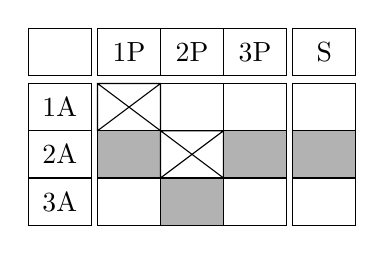
\begin{tikzpicture}[xscale=.8, yscale=-.6, draw=black, fill=black!30]
	\draw     (-.1,-.17) node{}   +(-.5,-.5) rectangle ++(.5,.5);
	\draw     (1,-.17)   node{1P} +(-.5,-.5) rectangle ++(.5,.5);
	\draw     (2,-.17)   node{2P} +(-.5,-.5) rectangle ++(.5,.5);
	\draw     (3,-.17)   node{3P} +(-.5,-.5) rectangle ++(.5,.5);
	\draw     (4.1,-.17) node{S}  +(-.5,-.5) rectangle ++(.5,.5);
	\draw     (-.1,1)    node{1A} +(-.5,-.5) rectangle ++(.5,.5);
	\draw     (1,1)      node{}   +(-.5,-.5) rectangle ++(.5,.5) -- ++(-1,-1) ++(0,1) -- ++(1,-1);
	\draw     (2,1)      node{}   +(-.5,-.5) rectangle ++(.5,.5);
	\draw     (3,1)      node{}   +(-.5,-.5) rectangle ++(.5,.5);
	\draw     (4.1,1)    node{}   +(-.5,-.5) rectangle ++(.5,.5);
	\draw     (-.1,2)    node{2A} +(-.5,-.5) rectangle ++(.5,.5);
	\filldraw (1,2)      node{}   +(-.5,-.5) rectangle ++(.5,.5);
	\draw     (2,2)      node{}   +(-.5,-.5) rectangle ++(.5,.5) -- ++(-1,-1) ++(0,1) -- ++(1,-1);
	\filldraw (3,2)      node{}   +(-.5,-.5) rectangle ++(.5,.5);
	\filldraw (4.1,2)    node{}   +(-.5,-.5) rectangle ++(.5,.5);
	\draw     (-.1,3)    node{3A} +(-.5,-.5) rectangle ++(.5,.5);
	\draw     (1,3)      node{}   +(-.5,-.5) rectangle ++(.5,.5);
	\filldraw (2,3)      node{}   +(-.5,-.5) rectangle ++(.5,.5);
	\draw     (3,3)      node{}   +(-.5,-.5) rectangle ++(.5,.5);
	\draw     (4.1,3)    node{}   +(-.5,-.5) rectangle ++(.5,.5);
\end{tikzpicture}\\
\emph{-ka} \rede{2} (neutral, except 1>2)
\end{minipage}
\begin{minipage}[t]{.4\textwidth}

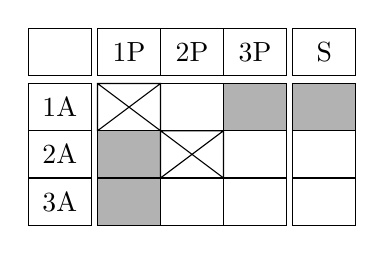
\begin{tikzpicture}[xscale=.8, yscale=-.6, draw=black, fill=black!30]
	\draw     (-.1,-.17) node{}   +(-.5,-.5) rectangle ++(.5,.5);
	\draw     (1,-.17)   node{1P} +(-.5,-.5) rectangle ++(.5,.5);
	\draw     (2,-.17)   node{2P} +(-.5,-.5) rectangle ++(.5,.5);
	\draw     (3,-.17)   node{3P} +(-.5,-.5) rectangle ++(.5,.5);
	\draw     (4.1,-.17) node{S}  +(-.5,-.5) rectangle ++(.5,.5);
	\draw     (-.1,1)    node{1A} +(-.5,-.5) rectangle ++(.5,.5);
	\draw     (1,1)      node{}   +(-.5,-.5) rectangle ++(.5,.5) -- ++(-1,-1) ++(0,1) -- ++(1,-1);
	\draw     (2,1)      node{}   +(-.5,-.5) rectangle ++(.5,.5);
	\filldraw (3,1)      node{}   +(-.5,-.5) rectangle ++(.5,.5);
	\filldraw (4.1,1)    node{}   +(-.5,-.5) rectangle ++(.5,.5);
	\draw     (-.1,2)    node{2A} +(-.5,-.5) rectangle ++(.5,.5);
	\filldraw (1,2)      node{}   +(-.5,-.5) rectangle ++(.5,.5);
	\draw     (2,2)      node{}   +(-.5,-.5) rectangle ++(.5,.5) -- ++(-1,-1) ++(0,1) -- ++(1,-1);
	\draw     (3,2)      node{}   +(-.5,-.5) rectangle ++(.5,.5);
	\draw     (4.1,2)    node{}   +(-.5,-.5) rectangle ++(.5,.5);
	\draw     (-.1,3)    node{3A} +(-.5,-.5) rectangle ++(.5,.5);
	\filldraw (1,3)      node{}   +(-.5,-.5) rectangle ++(.5,.5);
	\draw     (2,3)      node{}   +(-.5,-.5) rectangle ++(.5,.5);
	\draw     (3,3)      node{}   +(-.5,-.5) rectangle ++(.5,.5);
	\draw     (4.1,3)    node{}   +(-.5,-.5) rectangle ++(.5,.5);
\end{tikzpicture}\\
\emph{-ŋ(a)} \rede{excl, 1sg} (neutral, except 1>2)
\end{minipage}
\\[.2em]

\begin{minipage}[t]{.4\textwidth}

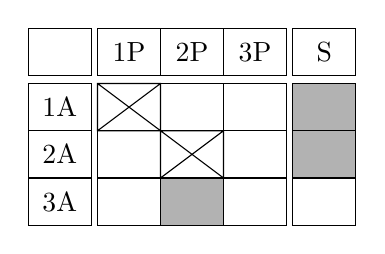
\begin{tikzpicture}[xscale=.8, yscale=-.6, draw=black, fill=black!30]
	\draw     (-.1,-.17) node{}   +(-.5,-.5) rectangle ++(.5,.5);
	\draw     (1,-.17)   node{1P} +(-.5,-.5) rectangle ++(.5,.5);
	\draw     (2,-.17)   node{2P} +(-.5,-.5) rectangle ++(.5,.5);
	\draw     (3,-.17)   node{3P} +(-.5,-.5) rectangle ++(.5,.5);
	\draw     (4.1,-.17) node{S}  +(-.5,-.5) rectangle ++(.5,.5);
	\draw     (-.1,1)    node{1A} +(-.5,-.5) rectangle ++(.5,.5);
	\draw     (1,1)      node{}   +(-.5,-.5) rectangle ++(.5,.5) -- ++(-1,-1) ++(0,1) -- ++(1,-1);
	\draw     (2,1)      node{}   +(-.5,-.5) rectangle ++(.5,.5);
	\draw     (3,1)      node{}   +(-.5,-.5) rectangle ++(.5,.5);
	\filldraw (4.1,1)    node{}   +(-.5,-.5) rectangle ++(.5,.5);
	\draw     (-.1,2)    node{2A} +(-.5,-.5) rectangle ++(.5,.5);
	\draw     (1,2)      node{}   +(-.5,-.5) rectangle ++(.5,.5);
	\draw     (2,2)      node{}   +(-.5,-.5) rectangle ++(.5,.5) -- ++(-1,-1) ++(0,1) -- ++(1,-1);
	\draw     (3,2)      node{}   +(-.5,-.5) rectangle ++(.5,.5);
	\filldraw (4.1,2)    node{}   +(-.5,-.5) rectangle ++(.5,.5);
	\draw     (-.1,3)    node{3A} +(-.5,-.5) rectangle ++(.5,.5);
	\draw     (1,3)      node{}   +(-.5,-.5) rectangle ++(.5,.5);
	\filldraw (2,3)      node{}   +(-.5,-.5) rectangle ++(.5,.5);
	\draw     (3,3)      node{}   +(-.5,-.5) rectangle ++(.5,.5);
	\draw     (4.1,3)    node{}   +(-.5,-.5) rectangle ++(.5,.5);
\end{tikzpicture}\\
\emph{-i} \rede{1/2pl.S} \& \rede{2P}  (ergative for 2, except 1>2)
\end{minipage}
\begin{minipage}[t]{.4\textwidth}

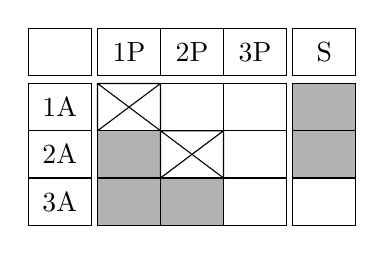
\begin{tikzpicture}[xscale=.8, yscale=-.6, draw=black, fill=black!30]
	\draw     (-.1,-.17) node{}   +(-.5,-.5) rectangle ++(.5,.5);
	\draw     (1,-.17)   node{1P} +(-.5,-.5) rectangle ++(.5,.5);
	\draw     (2,-.17)   node{2P} +(-.5,-.5) rectangle ++(.5,.5);
	\draw     (3,-.17)   node{3P} +(-.5,-.5) rectangle ++(.5,.5);
	\draw     (4.1,-.17) node{S}  +(-.5,-.5) rectangle ++(.5,.5);
	\draw     (-.1,1)    node{1A} +(-.5,-.5) rectangle ++(.5,.5);
	\draw     (1,1)      node{}   +(-.5,-.5) rectangle ++(.5,.5) -- ++(-1,-1) ++(0,1) -- ++(1,-1);
	\draw     (2,1)      node{}   +(-.5,-.5) rectangle ++(.5,.5);
	\draw     (3,1)      node{}   +(-.5,-.5) rectangle ++(.5,.5);
	\filldraw (4.1,1)    node{}   +(-.5,-.5) rectangle ++(.5,.5);
	\draw     (-.1,2)    node{2A} +(-.5,-.5) rectangle ++(.5,.5);
	\filldraw (1,2)      node{}   +(-.5,-.5) rectangle ++(.5,.5);
	\draw     (2,2)      node{}   +(-.5,-.5) rectangle ++(.5,.5) -- ++(-1,-1) ++(0,1) -- ++(1,-1);
	\draw     (3,2)      node{}   +(-.5,-.5) rectangle ++(.5,.5);
	\filldraw (4.1,2)    node{}   +(-.5,-.5) rectangle ++(.5,.5);
	\draw     (-.1,3)    node{3A} +(-.5,-.5) rectangle ++(.5,.5);
	\filldraw (1,3)      node{}   +(-.5,-.5) rectangle ++(.5,.5);
	\filldraw (2,3)      node{}   +(-.5,-.5) rectangle ++(.5,.5);
	\draw     (3,3)      node{}   +(-.5,-.5) rectangle ++(.5,.5);
	\draw     (4.1,3)    node{}   +(-.5,-.5) rectangle ++(.5,.5);
\end{tikzpicture}\\
Historical forms (recent loss of 1nsg.P forms): \emph{-i} \rede{1/2pl.S/P} (ergative)
\end{minipage}\\[.2em]

\begin{minipage}[t]{.4\textwidth}

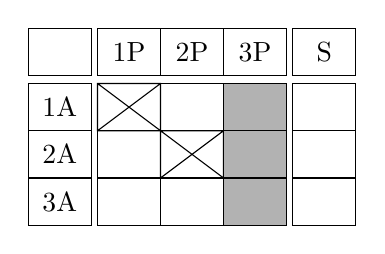
\begin{tikzpicture}[xscale=.8, yscale=-.6, draw=black, fill=black!30]
	\draw     (-.1,-.17) node{}   +(-.5,-.5) rectangle ++(.5,.5);
	\draw     (1,-.17)   node{1P} +(-.5,-.5) rectangle ++(.5,.5);
	\draw     (2,-.17)   node{2P} +(-.5,-.5) rectangle ++(.5,.5);
	\draw     (3,-.17)   node{3P} +(-.5,-.5) rectangle ++(.5,.5);
	\draw     (4.1,-.17) node{S}  +(-.5,-.5) rectangle ++(.5,.5);
	\draw     (-.1,1)    node{1A} +(-.5,-.5) rectangle ++(.5,.5);
	\draw     (1,1)      node{}   +(-.5,-.5) rectangle ++(.5,.5) -- ++(-1,-1) ++(0,1) -- ++(1,-1);
	\draw     (2,1)      node{}   +(-.5,-.5) rectangle ++(.5,.5);
	\filldraw (3,1)      node{}   +(-.5,-.5) rectangle ++(.5,.5);
	\draw     (4.1,1)    node{}   +(-.5,-.5) rectangle ++(.5,.5);
	\draw     (-.1,2)    node{2A} +(-.5,-.5) rectangle ++(.5,.5);
	\draw     (1,2)      node{}   +(-.5,-.5) rectangle ++(.5,.5);
	\draw     (2,2)      node{}   +(-.5,-.5) rectangle ++(.5,.5) -- ++(-1,-1) ++(0,1) -- ++(1,-1);
	\filldraw (3,2)      node{}   +(-.5,-.5) rectangle ++(.5,.5);
	\draw     (4.1,2)    node{}   +(-.5,-.5) rectangle ++(.5,.5);
	\draw     (-.1,3)    node{3A} +(-.5,-.5) rectangle ++(.5,.5);
	\draw     (1,3)      node{}   +(-.5,-.5) rectangle ++(.5,.5);
	\draw     (2,3)      node{}   +(-.5,-.5) rectangle ++(.5,.5);
	\filldraw (3,3)      node{}   +(-.5,-.5) rectangle ++(.5,.5);
	\draw     (4.1,3)    node{}   +(-.5,-.5) rectangle ++(.5,.5);
\end{tikzpicture}\\
\emph{-u} \rede{3P}, \emph{-ci} \rede{3nsg.P}  (accusative)
\end{minipage}
\begin{minipage}[t]{.4\textwidth}

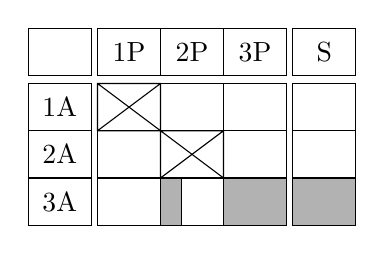
\begin{tikzpicture}[xscale=.8, yscale=-.6, draw=black, fill=black!30]
	\draw     (-.1,-.17) node{}   ++(-.5,-.5) rectangle ++(1,1);
	\draw     (1,-.17)   node{1P} ++(-.5,-.5) rectangle ++(1,1);
	\draw     (2,-.17)   node{2P} ++(-.5,-.5) rectangle ++(1,1);
	\draw     (3,-.17)   node{3P} ++(-.5,-.5) rectangle ++(1,1);
	\draw     (4.1,-.17) node{S}  ++(-.5,-.5) rectangle ++(1,1);
	\draw     (-.1,1)    node{1A} ++(-.5,-.5) rectangle ++(1,1);
	\draw     (1,1)      node{}   ++(-.5,-.5) rectangle ++(1,1) -- ++(-1,-1) ++(0,1) -- ++(1,-1);
	\draw     (2,1)      node{}   ++(-.5,-.5) rectangle ++(1,1);
	\draw     (3,1)      node{}   ++(-.5,-.5) rectangle ++(1,1);
	\draw     (4.1,1)    node{}   ++(-.5,-.5) rectangle ++(1,1);
	\draw     (-.1,2)    node{2A} ++(-.5,-.5) rectangle ++(1,1);
	\draw     (1,2)      node{}   ++(-.5,-.5) rectangle ++(1,1);
	\draw     (2,2)      node{}   ++(-.5,-.5) rectangle ++(1,1) -- ++(-1,-1) ++(0,1) -- ++(1,-1);
	\draw     (3,2)      node{}   ++(-.5,-.5) rectangle ++(1,1);
	\draw     (4.1,2)    node{}   ++(-.5,-.5) rectangle ++(1,1);
	\draw     (-.1,3)    node{3A} ++(-.5,-.5) rectangle ++(1,1);
	\draw     (1,3)      node{}   ++(-.5,-.5) rectangle ++(1,1);
	\draw     (2,3)      node{}   ++(-.5,-.5) rectangle ++(1,1);
	\filldraw (3,3)      node{}   ++(-.5,-.5) rectangle ++(1,1);
	\filldraw (4.1,3)    node{}   ++(-.5,-.5) rectangle ++(1,1);
	%geteilt
	\filldraw (2,3)      node{}   ++(-.5,-.5) rectangle ++(.33,1);
\end{tikzpicture}\\
\emph{N-} \rede{3pl.S/A}, zero \rede{3sg.S/A} (accusative)
\end{minipage}\\[.2em]

\begin{minipage}[t]{.4\textwidth}

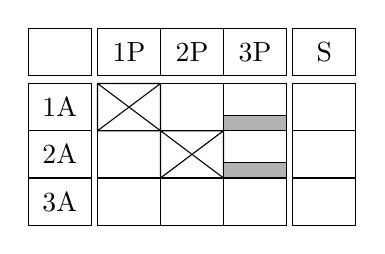
\begin{tikzpicture}[xscale=.8, yscale=-.6, draw=black, fill=black!30]
	\draw     (-.1,-.17) node{}   ++(-.5,-.5) rectangle ++(1,1);
	\draw     (1,-.17)   node{1P} ++(-.5,-.5) rectangle ++(1,1);
	\draw     (2,-.17)   node{2P} ++(-.5,-.5) rectangle ++(1,1);
	\draw     (3,-.17)   node{3P} ++(-.5,-.5) rectangle ++(1,1);
	\draw     (4.1,-.17) node{S}  ++(-.5,-.5) rectangle ++(1,1);
	\draw     (-.1,1)    node{1A} ++(-.5,-.5) rectangle ++(1,1);
	\draw     (1,1)      node{}   ++(-.5,-.5) rectangle ++(1,1) -- ++(-1,-1) ++(0,1) -- ++(1,-1);
	\draw     (2,1)      node{}   ++(-.5,-.5) rectangle ++(1,1);
	\draw     (3,1)      node{}   ++(-.5,-.5) rectangle ++(1,1);
	\draw     (4.1,1)    node{}   ++(-.5,-.5) rectangle ++(1,1);
	\draw     (-.1,2)    node{2A} ++(-.5,-.5) rectangle ++(1,1);
	\draw     (1,2)      node{}   ++(-.5,-.5) rectangle ++(1,1);
	\draw     (2,2)      node{}   ++(-.5,-.5) rectangle ++(1,1) -- ++(-1,-1) ++(0,1) -- ++(1,-1);
	\draw     (3,2)      node{}   ++(-.5,-.5) rectangle ++(1,1);
	\draw     (4.1,2)    node{}   ++(-.5,-.5) rectangle ++(1,1);
	\draw     (-.1,3)    node{3A} ++(-.5,-.5) rectangle ++(1,1);
	\draw     (1,3)      node{}   ++(-.5,-.5) rectangle ++(1,1);
	\draw     (2,3)      node{}   ++(-.5,-.5) rectangle ++(1,1);
	\draw     (3,3)      node{}   ++(-.5,-.5) rectangle ++(1,1);
	\draw     (4.1,3)    node{}   ++(-.5,-.5) rectangle ++(1,1);
	%geteilt
	\filldraw (3,1)      node{}   ++(-.5,.5) rectangle ++(1,-.33);
	\filldraw (3,2)      node{}   ++(-.5,.5) rectangle ++(1,-.33);
\end{tikzpicture}\\
\emph{-m} \rede{1/2pl>3} (scenario-portmanteau)
\end{minipage}
\begin{minipage}[t]{.4\textwidth}

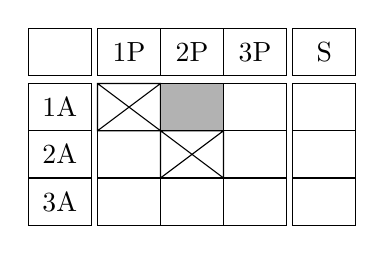
\begin{tikzpicture}[xscale=.8, yscale=-.6, draw=black, fill=black!30]
	\draw     (-.1,-.17) node{}   ++(-.5,-.5) rectangle ++(1,1);
	\draw     (1,-.17)   node{1P} ++(-.5,-.5) rectangle ++(1,1);
	\draw     (2,-.17)   node{2P} ++(-.5,-.5) rectangle ++(1,1);
	\draw     (3,-.17)   node{3P} ++(-.5,-.5) rectangle ++(1,1);
	\draw     (4.1,-.17) node{S}  ++(-.5,-.5) rectangle ++(1,1);
	\draw     (-.1,1)    node{1A} ++(-.5,-.5) rectangle ++(1,1);
	\draw     (1,1)      node{}   ++(-.5,-.5) rectangle ++(1,1) -- ++(-1,-1) ++(0,1) -- ++(1,-1);
	\filldraw (2,1)      node{}   ++(-.5,-.5) rectangle ++(1,1);
	\draw     (3,1)      node{}   ++(-.5,-.5) rectangle ++(1,1);
	\draw     (4.1,1)    node{}   ++(-.5,-.5) rectangle ++(1,1);
	\draw     (-.1,2)    node{2A} ++(-.5,-.5) rectangle ++(1,1);
	\draw     (1,2)      node{}   ++(-.5,-.5) rectangle ++(1,1);
	\draw     (2,2)      node{}   ++(-.5,-.5) rectangle ++(1,1) -- ++(-1,-1) ++(0,1) -- ++(1,-1);
	\draw     (3,2)      node{}   ++(-.5,-.5) rectangle ++(1,1);
	\draw     (4.1,2)    node{}   ++(-.5,-.5) rectangle ++(1,1);
	\draw     (-.1,3)    node{3A} ++(-.5,-.5) rectangle ++(1,1);
	\draw     (1,3)      node{}   ++(-.5,-.5) rectangle ++(1,1);
	\draw     (2,3)      node{}   ++(-.5,-.5) rectangle ++(1,1);
	\draw     (3,3)      node{}   ++(-.5,-.5) rectangle ++(1,1);
	\draw     (4.1,3)    node{}   ++(-.5,-.5) rectangle ++(1,1);
\end{tikzpicture}\\
\emph{-nen} \rede{1>2} (scenario-portmanteau)
\end{minipage}\\[.2em]

\begin{minipage}[t]{.4\textwidth}

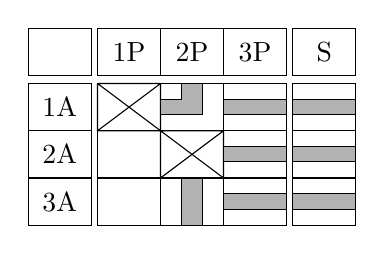
\begin{tikzpicture}[xscale=.8, yscale=-.6, draw=black, fill=black!30]
	\draw     (-.1,-.17) node{}   ++(-.5,-.5) rectangle ++(1,1);
	\draw     (1,-.17)   node{1P} ++(-.5,-.5) rectangle ++(1,1);
	\draw     (2,-.17)   node{2P} ++(-.5,-.5) rectangle ++(1,1);
	\draw     (3,-.17)   node{3P} ++(-.5,-.5) rectangle ++(1,1);
	\draw     (4.1,-.17) node{S}  ++(-.5,-.5) rectangle ++(1,1);
	\draw     (-.1,1)    node{1A} ++(-.5,-.5) rectangle ++(1,1);
	\draw     (1,1)      node{}   ++(-.5,-.5) rectangle ++(1,1) -- ++(-1,-1) ++(0,1) -- ++(1,-1);
	\draw     (2,1)      node{}   ++(-.5,-.5) rectangle ++(1,1);
	\draw     (3,1)      node{}   ++(-.5,-.5) rectangle ++(1,1);
	\draw     (4.1,1)    node{}   ++(-.5,-.5) rectangle ++(1,1);
	\draw     (-.1,2)    node{2A} ++(-.5,-.5) rectangle ++(1,1);
	\draw     (1,2)      node{}   ++(-.5,-.5) rectangle ++(1,1);
	\draw     (2,2)      node{}   ++(-.5,-.5) rectangle ++(1,1) -- ++(-1,-1) ++(0,1) -- ++(1,-1);
	\draw     (3,2)      node{}   ++(-.5,-.5) rectangle ++(1,1);
	\draw     (4.1,2)    node{}   ++(-.5,-.5) rectangle ++(1,1);
	\draw     (-.1,3)    node{3A} ++(-.5,-.5) rectangle ++(1,1);
	\draw     (1,3)      node{}   ++(-.5,-.5) rectangle ++(1,1);
	\draw     (2,3)      node{}   ++(-.5,-.5) rectangle ++(1,1);
	\draw     (3,3)      node{}   ++(-.5,-.5) rectangle ++(1,1);
	\draw     (4.1,3)    node{}   ++(-.5,-.5) rectangle ++(1,1);
	%geteilt
	\filldraw (2,1)      ++(-.5,-.5) ++(.33,0)--++(.33,0)--++(0,.66)--++(-.66,0)--++(0,-.33)--++(.33,0)--++(0,-.33);
	\filldraw (3,1)      ++(-.5,-.5) ++(0,.33) rectangle ++(1,.33);
	\filldraw (4.1,1)    ++(-.5,-.5) ++(0,.33) rectangle ++(1,.33);
	\filldraw (3,2)      ++(-.5,-.5) ++(0,.33) rectangle ++(1,.33);
	\filldraw (4.1,2)    ++(-.5,-.5) ++(0,.33) rectangle ++(1,.33);
	\filldraw (3,3)      ++(-.5,-.5) ++(0,.33) rectangle ++(1,.33);
	\filldraw (4.1,3)    ++(-.5,-.5) ++(0,.33) rectangle ++(1,.33);
	\filldraw (2,3)      ++(-.5,-.5) ++(.33,0) rectangle ++(.33,1);
\end{tikzpicture}\\
\emph{-ci} \rede{dual} (mixed: acc./neutral/ref.-based)
\end{minipage}
\begin{minipage}[t]{.4\textwidth}

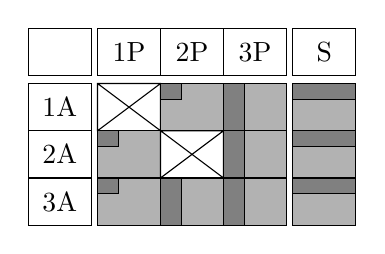
\begin{tikzpicture}[xscale=.8, yscale=-.6, draw=black, fill=black!30]
	\draw     (-.1,-.17) node{}   ++(-.5,-.5) rectangle ++(1,1);
	\draw     (1,-.17)   node{1P} ++(-.5,-.5) rectangle ++(1,1);
	\draw     (2,-.17)   node{2P} ++(-.5,-.5) rectangle ++(1,1);
	\draw     (3,-.17)   node{3P} ++(-.5,-.5) rectangle ++(1,1);
	\draw     (4.1,-.17) node{S}  ++(-.5,-.5) rectangle ++(1,1);
	\draw     (-.1,1)    node{1A} ++(-.5,-.5) rectangle ++(1,1);
	\draw     (1,1)      node{}   ++(-.5,-.5) rectangle ++(1,1) -- ++(-1,-1) ++(0,1) -- ++(1,-1);
	\filldraw (2,1)      node{}   ++(-.5,-.5) rectangle ++(1,1);
	\filldraw (3,1)      node{}   ++(-.5,-.5) rectangle ++(1,1);
	\filldraw (4.1,1)    node{}   ++(-.5,-.5) rectangle ++(1,1);
	\draw     (-.1,2)    node{2A} ++(-.5,-.5) rectangle ++(1,1);
	\filldraw (1,2)      node{}   ++(-.5,-.5) rectangle ++(1,1);
	\draw     (2,2)      node{}   ++(-.5,-.5) rectangle ++(1,1) -- ++(-1,-1) ++(0,1) -- ++(1,-1);
	\filldraw (3,2)      node{}   ++(-.5,-.5) rectangle ++(1,1);
	\filldraw (4.1,2)    node{}   ++(-.5,-.5) rectangle ++(1,1);
	\draw     (-.1,3)    node{3A} ++(-.5,-.5) rectangle ++(1,1);
	\filldraw (1,3)      node{}   ++(-.5,-.5) rectangle ++(1,1);
	\filldraw (2,3)      node{}   ++(-.5,-.5) rectangle ++(1,1);
	\filldraw (3,3)      node{}   ++(-.5,-.5) rectangle ++(1,1);
	\filldraw (4.1,3)    node{}   ++(-.5,-.5) rectangle ++(1,1);
	%entspricht =na (in hellerem Grau)
	\begin{scope}[fill=black!50]
	\filldraw (2,1)      ++(-.5,-.5) rectangle ++(.33,.33);
	\filldraw (1,2)      ++(-.5,-.5) rectangle ++(.33,.33);
	\filldraw (1,3)      ++(-.5,-.5) rectangle ++(.33,.33);
	\filldraw (3,1)      ++(-.5,-.5) rectangle ++(.33,1);
	\filldraw (3,2)      ++(-.5,-.5) rectangle ++(.33,1);
	\filldraw (3,3)      ++(-.5,-.5) rectangle ++(.33,1);
	\filldraw (2,3)      ++(-.5,-.5) rectangle ++(.33,1);
	\filldraw (4.1,1)    ++(-.5,-.5) rectangle ++(1,.33);
	\filldraw (4.1,2)    ++(-.5,-.5) rectangle ++(1,.33);
	\filldraw (4.1,3)    ++(-.5,-.5) rectangle ++(1,.33);
	\end{scope}
\end{tikzpicture}\\
\emph{=na} \rede{sg}; \emph{=ha} \rede{nsg} (mixed: erg./ref.-based)
\end{minipage}
\caption{The alignment of individual person/number markers}\label{aligntables}
\end{figure}




%\end{document}